\documentclass[a4paper,12pt]{report}
\usepackage{times,amsmath,amsthm,amssymb,graphicx,color,listings}
\usepackage[left=3cm,right=2cm,top=2.5cm,bottom=3.5cm]{geometry}

\definecolor{Brown}{cmyk}{0,0.81,1,0.60}
\definecolor{OliveGreen}{cmyk}{0.64,0,0.95,0.40}
\definecolor{CadetBlue}{cmyk}{0.52,0.57,0.23,0}
\definecolor{Yellow}{rgb}{0.8,0.8,0}
\definecolor{Black}{rgb}{0,0,0}
\definecolor{Red}{rgb}{0.8,0,0}
\lstset{language=bash}
\lstset{frame=ltrb,framesep=5pt,basicstyle=\small,
    keywordstyle=[1]\ttfamily\color{Black},
    identifierstyle=\ttfamily\color{Black},
    commentstyle=\color{CadetBlue},
    stringstyle=\color{Red}\ttfamily,
    showstringspaces=false
}
\numberwithin{equation}{section}
\setcounter{tocdepth}{3}
\setcounter{secnumdepth}{4}
\bibliographystyle{plain}

\begin{document}
\title{RaW Digital Playout System}
\author{Manual}
\date{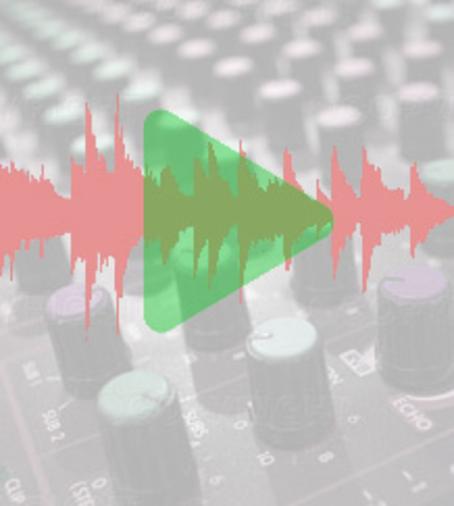
\includegraphics{digiplay.pdf}}
%\date{\today}
\maketitle

\clearpage

\chapter{Introduction}
Welcome to RaW's digital playout system (DPS) \emph{Digiplay}. This open-source project aims to ultimately develop a full suite of software for providing digital playout and automation services for radio stations of any size. The primary goal is to provide a simple, yet effective interface by which users can access digitally stored audio.

\emph{Digiplay} comprises several software applications, a web application and a suite of management tools, all of which operate using a central database. These are:
\begin{itemize}
\item Studio Playout Application\par
Provides three audio players, a station audio wall and a user audio wall. Separates broadcast playout from management to improve reliability.
\item Studio Management Application\par
Provides facilities to generate a show plan by searching the music library, or selecting tracks from a playlist or virtual directory system. Also provides access to studio emails and logging features.
\item DPS Website \& Administrative Interface\par
Allows users to log in remotely and create show plans or audio sets (for use with the user audio wall). Users can be granted privilages to perform different administrative tasks, such as user/group management, music library management, modify sustainer service playlist and edit the station audio set.
\item Automated Sustainer Service (Sue)\par
A (simple) automated sustainer service which plays out music from the system as specified in the sustainer playlist.
\item Audio Acquisition Tool\par
Simple tool for accurately extracting and cataloguing audio from CDs onto the system using CD Paranoia.
\item DPS Management Tools\par
Set of command-line tools for backend management of the system.
\end{itemize}
This document describes an installation procedure to suite the majority of system configurations.

\chapter{Choosing a System Configuration}
Before beginning, it is advisable to first plan how the software will be deploed. This will depend on the size of the radio station that the software will serve, as well as the availability of hardware. Some basic things to consider are:
\begin{itemize}
\item How many studios will the system support?
\item How much audio will the system store?
\item How many users will the system support?
\end{itemize}
Planning the system now may reduce possibly complications later as the system expands and develops.

\section{Audio Storage}
Audio is stored in raw PCM format (and soon using FLAC compression), to provide the highest quality output. Raw PCM audio uses 10.56MB/min, so around 40MB will be required for an average four minute track. On a consumer 200GB hard disk, this equates to just under 5000 tracks. Audio can be written to any mounted local or remote linux file system. Multiple storage \emph{archives} are supported allowing, for instance, multiple disk arrays on multiple servers to be used thus permitting indefinite expansion of the system. While archives may be moved as a whole, the software does not currently support the redistribution of individual tracks. Potential storage configurations are:
\begin{enumerate}
\item Local storage on studio machine. This may be the addition of a pair of 200GB hard disks in the studio playout machine for example.
\item Remote storage on an existing generic file server. You can use any existing storage volume which can be exported over NFS.
\item Dedicated remote storage on multiple NAS, dedicated playout servers or SAN.
\end{enumerate}
The first two options are suitable for small installations with one or two studios. Audio can be initially stored on an existing storage volume, and then moved to dedicated storage at a later date as the archive outgrows this volume. This permits the distribution of hardware costs. The third option is appropriate for larger installations with many studios or large storage requirements (e.g. more than 10,000 tracks), who can finance and support this enterprise-class hardware.
\textbf{Note:} It is advisable to use data redundancy techniques, such as RAID1 or RAID5 to reduce the likelihood of data loss. Ideally the audio data should be regularly mirrored to a server located in a different building, or backed up to another medium and stored elsewhere. These are, of course, standard data protection measures.

\section{Database}
The central database may be located on any host, but must be accessible by every playout system. If there is a dedicated server for audio storage, it is advisable to install the database on that machine. For single or dual studio configurations the database may be installed on one of the studio machines without significant performance penalties, as the database load will not be significant.

\section{Studio Software}
There are two components to the studio software: a management interface, and a playout interface. These may either be run on separate physical systems, or together on the one system using two X servers. A separate physical display is required for each application. It is recommended to use a touch screen for the playout application.

\section{Hardware Requirements}
The system was designed to use commonly available consumer hardware wherever possible to minimise hardware costs. The main exception is the studio playout software, for which a touchscreen is recommended. The studio playout software can still be operated using a conventional keyboard and mouse.

\chapter{Installation}
Installation consists of the following tasks. We will assume the use of a Debian based distribution, but other distributions will follow a similar procedure.
\begin{enumerate}
\item Preliminaries: download and unpacking the software.
\item Install and configure the backend database.
\item Compile and install the management tools and set up an audio store.
\item Compile and install the audio acquisition software.
\item Compile and install the studio software.
\end{enumerate}

\section{Preliminaries}
Download the latest version of digiplay onto every digital playout computer. This guide will assume it has been downloaded to \texttt{/usr/local/src}. As root (replace $<$release$>$ with the latest version),
\begin{lstlisting}
cd /usr/local/src
tar -zxvf digiplay_<release>.tar.gz
cd digiplay
\end{lstlisting}
The \texttt{INSTALL} file contains a more detailed description of the archive contents, including a full list of package dependancies.

\section{Install and Configure backend database}
This must be installed on one machine only. The database uses the PostgreSQL database engine.
\begin{enumerate}
\item Install the database server (it is recommended to use PostgreSQL 8.0 or later).
\begin{lstlisting}
apt-get update
apt-get install postgresql-8.1 postgresql-client-8.1
\end{lstlisting}
This will most likely install additional dependancies. The configuration of the PostgreSQL server itself is beyond the scope of this document. Of particular importance is the configuration of the \texttt{pg\_hba.conf} file if the system configuration chosen consists of multiple hosts. For ease of installation, it is recommended to add a suitable line to trust the digiplay\_user access to the digiplay database from your local network. Security can be improved upon successful installation. For example,
\begin{lstlisting}
host     digiplay     digiplay_user    192.168.1.0/24    trust
\end{lstlisting}
\item Install the \texttt{/etc/digiplay.conf} configuration file.
\begin{lstlisting}
cp doc/digiplay.conf /etc/
\end{lstlisting}
This should be correct for the default installation on the machine running the database server. The database and users specified will be created in the next step.
\item Run the database install script: \texttt{dpsinstall}
\begin{lstlisting}
cd /usr/local/src/digiplay/db
./dpsinstall
\end{lstlisting}
This will parse the configuration file and create the database and required database users.
\end{enumerate}

\section{Compile and Install Management Tools}
The management tools perform administrative functions on the system. They are generally installed on the host serving the database, although this is not mandatory.
\begin{enumerate}
\item Install dependancies
\begin{lstlisting}
apt-get update
apt-get install libreadline-dev libpqxx-dev	make g++
\end{lstlisting}
This may install additional packages required by the above.
\item Compile and install the tools. By default applications are installed in \texttt{/usr/local/bin} and libraries in \texttt{/usr/local/lib}, but this may be altered by editing the \texttt{Makefile} in the root of the digiplay package.
\begin{lstlisting}
cd /usr/local/src/digiplay
make tools
make install
\end{lstlisting}
\item Create an audio archive. You may specify a descriptive name for each audio archive. If this audio archive will not be located on the database host, then it must be mounted over NFS on all digital playout hosts.\par
\textbf{NOTE:} The mount point MUST be consistently named across all hosts.\par
You may list the available audio archives using the same tool.
\begin{lstlisting}
dpsarchive -A "Music1" -l "/mnt/audio1" \
	-r "server:/export/audio1"
dpsarchive -L
\end{lstlisting}
\end{enumerate}

\section{Install the Audio Acquisition software}
This is used to transfer music from CD's onto the system. It simply requires a machine with a CDROM drive.
\begin{enumerate}
\item Install dependancies.
\begin{lstlisting}
apt-get install libreadline-dev make g++
\end{lstlisting}
\item Compile and install the software.
\begin{lstlisting}
make playin
make install
\end{lstlisting}
\end{enumerate}

\section{Install the Studio Software}
There are two components to the studio software. 
\subsection{Studio Management}
\begin{enumerate}
\item Install and configure an X server. This is outside the scope of this document. A window manager is not required (nor recommended). The studio software applications should be set to start automatically when the X server starts. The screen resolution should be set to 1024x768.
\item Install dependancies
\begin{lstlisting}
apt-get update
apt-get install libpqxx-dev	libldap2-dev libqt3-mt-dev \
     make g++
\end{lstlisting}
\item Create a non-privilaged user account, \texttt{digiplay}, for the studio software.
\item Compile and install the \texttt{studio\_manage} application.
\begin{lstlisting}
make studio_manage install
\end{lstlisting}
\item Install and modify the configuration file.
\begin{lstlisting}
cp doc/digiplay.conf /etc/
\end{lstlisting}
The \texttt{digiplay.conf} file should now be edited to correctly identify the central database set up earlier by specifying the correct host and port (and database name if you chose a different name).
\end{enumerate}
\subsection{Studio Playout}
\begin{enumerate}
\item Install dependancies
\begin{lstlisting}
apt-get update
apt-get install libpqxx-dev libqt3-mt-dev make g++
\end{lstlisting}
\item Create a non-privilaged user account, \texttt{digiplay}, for the studio software.
\item Compile and install the \texttt{studio\_play} application.
\begin{lstlisting}
make studio_play install
\end{lstlisting}
\item Install and modify the configuration as done previously.
\end{enumerate}

\section{Other Features}
\subsection{Studio Email support}
To enable studio emails, the incoming emails must be transfered to the DPS database by your Mail Transfer Agent (MTA). The \texttt{scripts} directory includes \texttt{dpsemail.pl} which receives email from your MTA (e.g. Exim), processes it and stores it in the database.
\begin{enumerate}
\item Install dependancies. The script is written in perl and uses database, email and mime perl libraries.
\begin{lstlisting}
apt-get update
apt-get install perl libmailtools-perl libmime-perl \
    libdbi-perl libdbd-pg-perl
\end{lstlisting}
This may install other packages on which these depend.
\item Copy the script to a suitable location (e.g. \texttt{/usr/local/bin}) which is accessible by the MTA. Ensure it has execute permissions. 
\begin{lstlisting}
cp /usr/local/src/digiplay/scripts/dpsemailpl /usr/local/bin
chmod +x /usr/local/bin/dpsemail.pl
\end{lstlisting}
\item Copy and configure the \texttt{/etc/digiplay.conf} file if this is not already present on the host which runs the MTA.
\item Instruct the MTA to pipe incoming emails to the script. For Exim, this would be done in the \texttt{/etc/aliases} file by adding the following line.
\begin{lstlisting}
cat >> /etc/aliases << EOF
studio: "|/usr/local/bin/dpsemail.pl"
EOF
\end{lstlisting}
\end{enumerate}

\chapter{Starting Digiplay}
\section{Studio Software}
The Studio software applications should be run from the running X servers \texttt{.xsession} file. A window manager is not required. For example,
\begin{lstlisting}
cat > /home/digiplay/.xsession << EOF
xset dpms 0 0 900
xset s off
exec /usr/local/bin/studio_play
EOF
\end{lstlisting}
This disables the DPMS standby and suspend states for the monitor, setting it to switch off after 15 minutes. It also disables the screensaver. Finally, it runs the studio software. If run as root, the studio software will drop to the unprivilaged \texttt{digiplay} user immediately. This may cause issues with X server permissions if the X server is not running as digiplay. Fix with
\begin{lstlisting}
xhost +digiplay
\end{lstlisting}
The X server should also use 75dpi fonts, rather than 100dpi. It may be necessary to edit \texttt{/etc/X11/xinit/xserverrc} to enforce this.
\textbf{Note:} The X server will terminate when the studio software terminates. If run from \texttt{/etc/inittab}, it will restart automatically.
\end{document}
